\documentclass[tikz,border=2pt]{standalone}
\usepackage{amsmath}
\usepackage{pgfplots}
\pgfplotsset{compat=1.18}
\usetikzlibrary{arrows.meta}
\begin{document}
% Logistic equation x' = x(1-x). Left: f(x) = x(1-x) with zeros 0 and 1 (the equilibria) and the
% phase line (f > 0 on (0,1): right; f < 0 outside: left). Right: the constant solutions 0 and 1 and
% the solutions x(t) = 1/(1+4e^{-t}) from x(0) = 0.2 and x(t) = 1/(1-e^{-t}/3) from x(0) = 1.5.
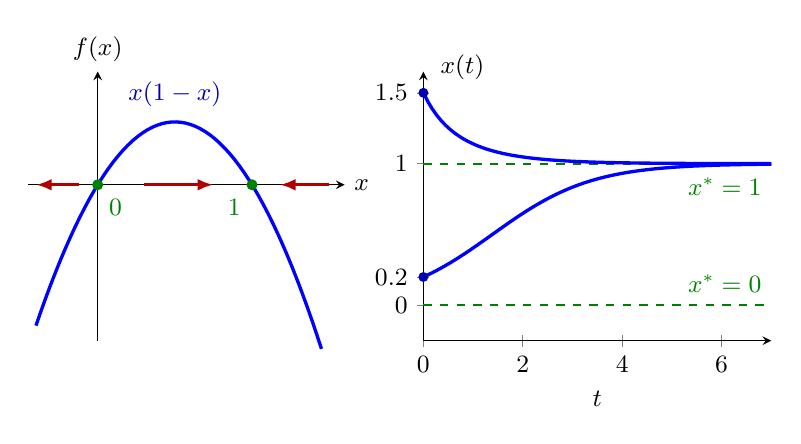
\begin{tikzpicture}[font=\small, >={Latex[length=2mm]}]
  \begin{axis}[
    name=phase, axis lines=middle, width=5.6cm, height=5.0cm,
    xmin=-0.45, xmax=1.6, ymin=-0.62, ymax=0.45,
    xtick=\empty, ytick=\empty, xlabel={$x$}, ylabel={$f(x)$},
    xlabel style={anchor=west}, ylabel style={anchor=south}, clip=false
    ]
    \addplot[blue, very thick, domain=-0.4:1.45, samples=60] {x*(1-x)};
    \draw[->, red!70!black, very thick] (axis cs:0.3,0) -- (axis cs:0.75,0);
    \draw[->, red!70!black, very thick] (axis cs:-0.12,0) -- (axis cs:-0.4,0);
    \draw[->, red!70!black, very thick] (axis cs:1.5,0) -- (axis cs:1.18,0);
    \fill[green!50!black] (axis cs:0,0) circle (2pt);
    \fill[green!50!black] (axis cs:1,0) circle (2pt);
    \node[green!50!black, anchor=north west] at (axis cs:0.01,-0.02) {$0$};
    \node[green!50!black, anchor=north east] at (axis cs:0.99,-0.02) {$1$};
    \node[blue!70!black, anchor=south] at (axis cs:0.5,0.27) {$x(1-x)$};
  \end{axis}
  \begin{axis}[
    at={(phase.east)}, anchor=west, xshift=1.0cm,
    axis lines=left, width=6.0cm, height=5.0cm,
    xmin=0, xmax=7, ymin=-0.25, ymax=1.65, xtick={0,2,4,6}, ytick={0,0.2,1,1.5},
    yticklabels={$0$,$0.2$,$1$,$1.5$}, xlabel={$t$}, clip=false, samples=80
    ]
    \addplot[green!50!black, thick, dashed, domain=0:7] {0};
    \addplot[green!50!black, thick, dashed, domain=0:7] {1};
    \addplot[blue, very thick, domain=0:7] {1/(1+4*exp(-x))};
    \addplot[blue, very thick, domain=0:7] {1/(1-exp(-x)/3)};
    \fill[blue!70!black] (axis cs:0,0.2) circle (1.8pt);
    \fill[blue!70!black] (axis cs:0,1.5) circle (1.8pt);
    \node[anchor=west] at (axis cs:0.15,1.68) {$x(t)$};
    \node[green!50!black, anchor=north east] at (axis cs:7,0.97) {$x^*=1$};
    \node[green!50!black, anchor=south east] at (axis cs:7,0.02) {$x^*=0$};
  \end{axis}
\end{tikzpicture}
\end{document}
